\section{Evaluatie}
\label{sec:eva}

\subsection{Resultaten}

\subsubsection{Deelvraag 1}
Het beste resultaat werd bereikt met Support Vector Machines gebruikmakend van \textit{stochastic gradient descent learning} en Elasticnet regularisatie. De features waren hierbij gestemd, met unigrams, bigrams en trigrams. Geen features zijn hierin weggelaten door minimale of maximale documentfrequenties. Het verschil in scores is zeer klein, zoals te zien in figuur XXX. In bijlage YYY staan uitgebreidere figuren over het effect van de classificatiemethoden. De scores zijn ruim hoger dan de baseline scores. De scores liggen binnen de scores gevonden in gerelateerd werk, ondanks dat de baseline scores aanzienlijk lager zijn en de documentgrootte kleiner is.\par
Tabel \ref{tab:classrapport} laat de scores zien per partij met het aantal documenten in de test set. De $F_1$ scores per partij liggen tussen de 0.7 en 0.8. De one-issuepartijen, 50PLUS en PvdD, hebben scores daarboven, terwijl de coalitiepartijen, VVD en PvdA, lagere scores hebben. Figuur \ref{fig:confusionmatrix} laat zien waar de fouten in deze classificatie zitten. De meest karakteristieke features per partij zijn te zien in tabel \ref{tab:MostImportantWords}. Hierin is te zien dat vrijwel alle woorden verwijzen naar de partij of een Kamerlid van die partij.\par

\begin{table}[H]
\caption{Classificatierapport van beste classificatie.}
\label{tab:classrapport}
\centering
\begin{tabular}{lrrrlr}
\toprule
{} &  Precision &  Recall &  F1\_score & Accuracy &  Documenten \\
\midrule
50PLUS       &       0.97 &    0.85 &      0.91 &        - &        71.4 \\
CDA          &       0.80 &    0.79 &      0.80 &        - &       379.6 \\
ChristenUnie &       0.83 &    0.76 &      0.79 &        - &       215.4 \\
D66          &       0.78 &    0.75 &      0.76 &        - &       381.8 \\
GroenLinks   &       0.89 &    0.73 &      0.80 &        - &       209.2 \\
PVV          &       0.82 &    0.88 &      0.85 &        - &       345.0 \\
PvdA         &       0.72 &    0.71 &      0.71 &        - &       377.4 \\
PvdD         &       0.86 &    0.87 &      0.86 &        - &        81.2 \\
SGP          &       0.87 &    0.84 &      0.86 &        - &       134.8 \\
SP           &       0.73 &    0.85 &      0.78 &        - &       453.2 \\
VVD          &       0.77 &    0.73 &      0.75 &        - &       331.0 \\
Totaal       &       0.79 &    0.79 &      0.79 &     0.79 &      2980.0 \\
\bottomrule
\end{tabular}

\end{table}


\begin{figure}[H]
  \centering
    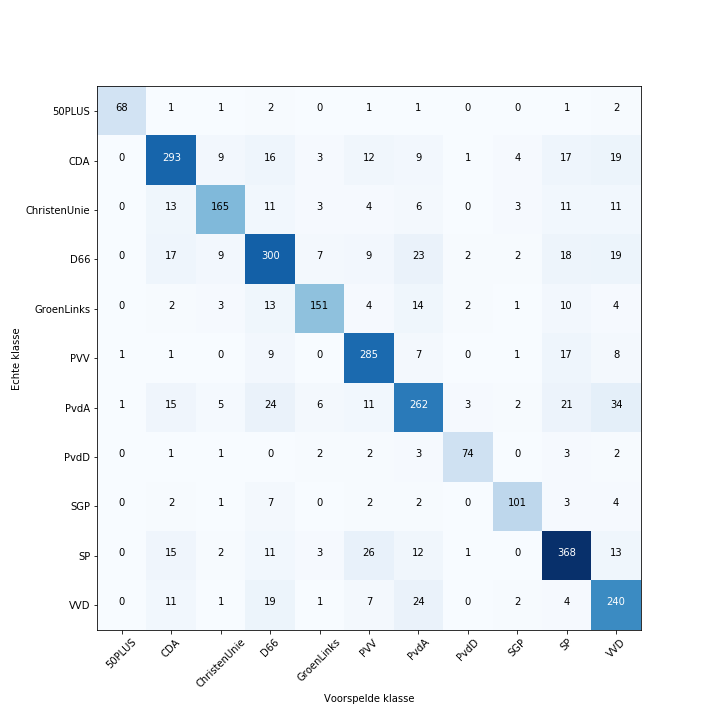
\includegraphics[width=0.60\paperwidth]{Verslag/Tables/confusionmatrix.png}
\caption{Confusion matrix van beste classificatie.}
\label{fig:confusionmatrix}
\end{figure}



\begin{table}[H]
\caption{Meest relevante woorden per partij op basis van beste classificatie gedurende kabinet-Rutte II.} 

\label{tab:MostImportantWords} 
\centering
\hspace*{-1in}
\begin{tabular}{lllll}
\toprule
          50PLUS &               CDA &         ChristenUnie &                  D66 &          GroenLinks \\
\midrule
          50plus &               cda &      de christenunie &                  d66 &          groenlinks \\
   lid krol naar &           het cda &         christenunie &         mijn fractie &    lid van tongeren \\
    het lid krol &            de cda &        lid dik faber &  leden van veldhoven &   lid voortman naar \\
        lid krol &       cda fractie &          het lid dik &       lid van meenen &    het lid voortman \\
   krol naar mij &    de cda fractie &              lid dik &        van veldhoven &        lid voortman \\
       krol naar &       lid omtzigt &            dik faber &            veldhoven &            voortman \\
            krol &   het lid omtzigt &                faber &    lid van veldhoven &            tongeren \\
      van 50plus &  lid omtzigt naar &     leden voordewind &         leden schouw &        van tongeren \\
 gepensioneerden &      omtzigt naar &  de leden voordewind &      de leden schouw &  leden van tongeren \\
         ouderen &  omtzigt naar mij &                  dik &               d66 is &   de leden voortman \\
\bottomrule
\end{tabular}
 
\end{table} 
\addtocounter{table}{-1} 
\begin{table}[H]
\caption{Meest relevante woorden per partij op basis van beste classificatie gedurende kabinet-Rutte II. \emph{(Vervolg)}} 
\centering
\hspace*{-1in}
\begin{tabular}{llllll}
\toprule
              PVV &             PvdA &              PvdD &              SGP &             SP &             VVD \\
\midrule
              pvv &          de pvda &      lid ouwehand &              sgp &             sp &          de vvd \\
           de pvv &             pvda &  lid ouwehand nar &           de sgp &          de sp &             vvd \\
      islamitisch &    de partij van &  het lid ouwehand &      sgp fractie &   lid van gerv &  de vvd fractie \\
        lid graus &    van de arbeid &      ouwehand nar &   de sgp fractie &     sp fractie &     vvd fractie \\
    het lid graus &        de arbeid &  ouwehand nar mij &     led dijkgraf &  de sp fractie &       de vvd is \\
    lid graus nar &    partij van de &          ouwehand &  de led dijkgraf &   van gerv nar &          vvd is \\
          miljard &       partij van &       vor de dier &      led van der &       gerv nar &      vor de vvd \\
    graus nar mij &     pvda fractie &           de dier &  de led bisschop &   gerv nar mij &      wat de vvd \\
        graus nar &           arbeid &              dier &     led bisschop &           gerv &     vvd betreft \\
 madlener nar mij &  de pvda fractie &     de partij vor &           sgp is &       van gerv &  de vvd betreft \\
\bottomrule
\end{tabular}
 
\end{table}

\subsubsection{Deelvraag 2}
In tabel \ref{tab:MostImportantWords} was al te zien dat de meest karakteristieke woorden voornamelijk bestaan uit partijnamen en namen van Kamerleden. In tabel \ref{tab:rapportwithoutnames} zijn de scores te zien van classificatie met partijnamen en namen van Kamerleden vervangen. In tabel \ref{tab:MostImportantWordsWithoutNames} is vervolgens te zien welke woorden het meest karakteristiek zijn per partij voor deze classificatie.
\begin{table}[H]
\caption{Classificatierapport van beste classificatie.}
\label{tab:rapportwithoutnames}
\centering
\begin{tabular}{lrrrlr}
\toprule
{} &  Precision &  Recall &  F1\_score & Accuracy &  Documenten \\
\midrule
50PLUS       &       0.97 &    0.85 &      0.91 &        - &        71.4 \\
CDA          &       0.80 &    0.79 &      0.80 &        - &       379.6 \\
ChristenUnie &       0.83 &    0.76 &      0.79 &        - &       215.4 \\
D66          &       0.78 &    0.75 &      0.76 &        - &       381.8 \\
GroenLinks   &       0.89 &    0.73 &      0.80 &        - &       209.2 \\
PVV          &       0.82 &    0.88 &      0.85 &        - &       345.0 \\
PvdA         &       0.72 &    0.71 &      0.71 &        - &       377.4 \\
PvdD         &       0.86 &    0.87 &      0.86 &        - &        81.2 \\
SGP          &       0.87 &    0.84 &      0.86 &        - &       134.8 \\
SP           &       0.73 &    0.85 &      0.78 &        - &       453.2 \\
VVD          &       0.77 &    0.73 &      0.75 &        - &       331.0 \\
Totaal       &       0.79 &    0.79 &      0.79 &     0.79 &      2980.0 \\
\bottomrule
\end{tabular}

\end{table}

\begin{table}[H] 
\caption{Meest relevante woorden per partij op basis van classificatie uit deelvraag 1 zonder partijnamen of namen van Kamerleden gedurende kabinet-Rutte II.} 
\label{tab:MostImportantWordsWithoutNames} 
\centering
\hspace*{-1in}
\begin{tabular}{lllll}
\toprule
                 50PLUS &             CDA &   ChristenUnie &           D66 &              GroenLinks \\
\midrule
        gepensioneerden &  PARTIJ fractie &   mensenhandel &  mijn fractie &                     zou \\
                ouderen &        inwoners &         zullen &          mijn &       kamer hierover te \\
                 oudere &          PARTIJ &       gezinnen &       fractie &     belastingontwijking \\
 koopkrachtontwikkeling &        regering &      inderdaad &    natuurlijk &            in elk geval \\
               plussers &             wij &  vluchtelingen &   het kabinet &        persoonsgebonden \\
                     50 &     de regering &       kinderen &    belangrijk &               elk geval \\
              werkenden &            hier &           hoop &       vandaag &                  in elk \\
            50 plussers &            echt &          motie &        kansen &  hierover te informeren \\
   voor gepensioneerden &         fractie &     onder meer &       kabinet &          schone energie \\
            overwegende &              de &     constateer &  buitengewoon &             hierover te \\
\bottomrule
\end{tabular}
 
\end{table} 
\addtocounter{table}{-1} 
\begin{table}[H] 
\caption{Meest relevante woorden per partij op basis van classificatie uit deelvraag 1 zonder partijnamen of namen van Kamerleden gedurende kabinet-Rutte II. \emph{(Vervolg)}} 
\centering
\hspace*{-0.6in}
\begin{tabular}{llllll}
\toprule
         PVV &             PvdA &              PvdD &                    SGP &            SP &            VVD \\
\midrule
 islamitisch &      mijn partij &              dier &               dank zer &       huurder &     volgen mij \\
       islam &       leerkracht &            de bio &  mevrouw de voorzitter &    segregatie &        liberal \\
     miljard &           tevred &     bio industrie &             mevrouw de &      herindel &      speelveld \\
    de islam &        circulair &               bio &           eenverdiener &        armoed &     verzekerar \\
 asielzoeker &   open standaard &        aan de bio &               allerlei &     de bevolk &          aruba \\
     brussel &          gezamen &  de bio industrie &                   punt &       jazeker &     ondernemer \\
   nederland &       ieder kind &            milieu &                 nadruk &          zegt &       regelgev \\
       grenz &  duurzam energie &     dierenwelzijn &                  woord &  bureaucratie &       aangegev \\
  immigratie &               en &          de natur &                 vanuit &     tenderned &  PARTIJNAAM is \\
          al &       lager over &   klimaatverander &                    oog &  ouderbijdrag &     essentieel \\
\bottomrule
\end{tabular}
 
\end{table}

\subsubsection{Deelvraag 3}
In figuur \ref{fig:distributies} zijn de distributies van de errors te zijn van combinaties tussen regerings- en oppositiepartijen.
\begin{figure}[H]
    \centering
    \hspace*{-0.2in}
    \subfloat[Tussen twee regeringspartijen]{{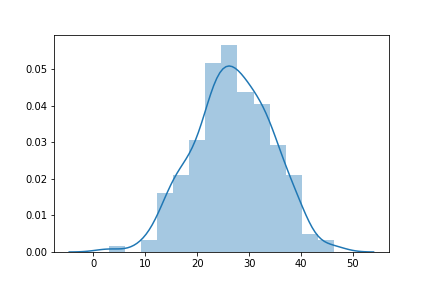
\includegraphics[width=7cm]{Verslag/Tables/Regering.png} }}%
    \subfloat[Tussen twee oppositiepartijen]{{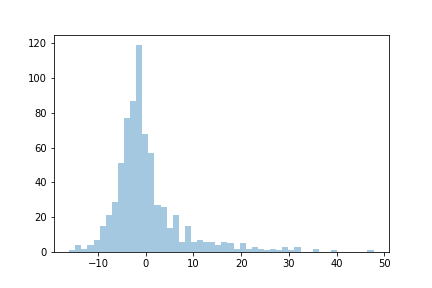
\includegraphics[width=7cm]{Verslag/Tables/Oppositie.png} }}\quad
    \hspace*{-0.2in}
    \subfloat[Tussen een regeringspartij en een oppositiepartij]{{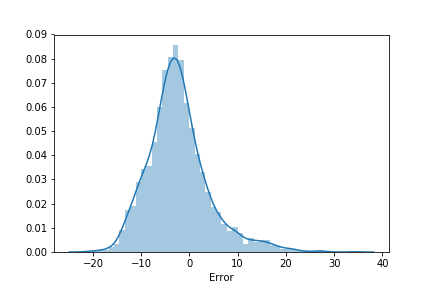
\includegraphics[width=7cm]{Verslag/Tables/Mix.png} }}%
    \subfloat[Totaal]{{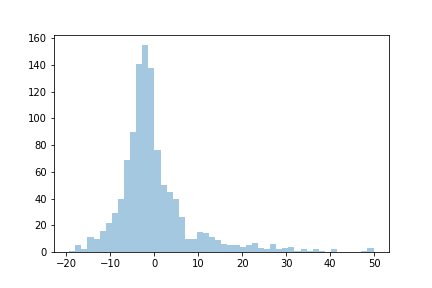
\includegraphics[width=7cm]{Verslag/Tables/Totaal.png} }}\quad
    \caption{Distributie van de error uit \ref{eq:error} voor de verschillende combinaties.}%
    \label{fig:distributies}%
\end{figure}

\subsection{Discussie}
\subsubsection{Deelvraag 1}
Het onderzoek behaalt resultaten in lijn der verwachting op basis van gerelateerd en daarnaast ruim boven de baseline scores.\par
Dit onderzoek heeft zich beperkt tot methoden genoemd in vergelijkbare onderzoeken en waarvan de implementatie beschikbaar is in scikit-learn. Een aantal methoden die in gerelateerde literatuur leidden tot goede classificaties zijn daarom niet getest. Ook nieuwe methoden die nog niet gebruikt zijn in een vergelijkbaar onderzoek voor politieke tekst classificatie zijn daarom niet getest. Daarnaast richtte zich dit ook maar op een beperkt aantal parameterwaarden. Een belangrijke hierbij is het maximaal iteraties, wat ver onder het aantal iteraties benodigd voor convergentie ligt. Voor vervolgonderzoek kan daarom dit onderdeel uitgebreid worden.\par
Het onderzoek van Hirst et al. vond dat resultaten afhankelijk kunnen zijn van documentgrootte. Alle documenten in dit onderzoek zijn kleiner dan de grootste documentgrootte uit het onderzoek van Hirst et al. en ook de minimumfrequentie lager ligt dan de kleinste documentgrootte uit dat onderzoek.
Het effect wat zij vinden tussen documentgrootte van 267 en 6666 is een verschil in nauwkeurigheid van 19,8\%. Voor een vervolgonderzoek kan gekeken worden naar of dit effect er is en wat dit betekent voor de resultaten.\par

\subsubsection{Deelvraag 2}
De resultaten laten zien dat de classificatie afhankelijk is van partijnamen en namen van Kamerleden.\par
De woorden in tabel \ref{tab:MostImportantWordsWithoutNames} komen bij veel partijen overeen met hun ideologie, vooral bij PVV, PvdD en 50PLUS. Daarnaast zijn er ook woorden die niet veel over ideologie zeggen, zoals; \textit{volgens mij}, \textit{ik constateer} en \textit{in elk geval}. Vooral de SGP heeft woorden die niet veel lijken te zeggen over de ideologie. Met name opvallend hierbij is \textit{mevrouw de voorzitter}, aangezien deze woorden door alle partijen gebruikt worden om via de voorzitter te praten. Voor een vervolgonderzoek kan gekeken naar waarom deze woorden zo karakteristiek zijn voor partijen. Een hypothese is dat deze woorden eigen zijn aan een individueel Kamerlid.\par
De classificatiemethode die gebruikt is in deze deelvraag, is gebaseerd op de beste methode voor de dataset uit deelvraag 1. Hierin was gevonden dat een combinatie van uni-, bi- en trigrams het beste resultaat opleverde. In tabel \ref{tab:MostImportantWords} is te zien dat trigrams behoren tot de meest karakteristieke woorden, hoewel de woorden in trigrams vaak overlappen met uni- en bigrams. In tabel \ref{tab:MostImportantWordsWithoutNames} daarentegen zijn er nog maar een paar trigrams, welke grotendeels procedurele zinnen zijn of toevoeging van een lidwoord op een uni- of bigram. Dit verschil suggereert dat trigrams minder belangrijk zijn in de classificatie zonder de namen, dus de classificatiemethode uit deelvraag 1 niet het beste is voor deze classificatie. In vervolgonderzoek kan de opzet van deelvraag 1 toegepast worden op de classificatie zonder de namen, om zo te komen tot een classificatiemethode die het beste resultaat oplevert op de classificatie zonder namen.\par 

\subsubsection{Deelvraag 3}
In tabel \ref{tab:classrapport} is het opvallend dat de coalitiepartijen lage scores krijgt. Daarnaast laat figuur \ref{fig:confusionmatrix} zien dat er een hoge overlap zit tussen deze twee partijen.\par

\subsubsection{Deelvraag 4}
Er zijn verschillende visies op links en rechts, en de indeling van de partijen, ook buiten de twee methoden gekozen in dit onderzoek.\par